% !TeX program = pdflatex


\documentclass[12pt]{article}
% for the equation* environment
\usepackage{amsmath}
\usepackage{amssymb}
\usepackage{amsthm}
\usepackage{amsfonts}

\usepackage{alphabeta}

\usepackage{csquotes}
\usepackage{subfigure}
\usepackage{float,lipsum}
\floatstyle{boxed}
\usepackage[top=3cm, bottom=3cm]{geometry}

\setlength{\footnotesep}{1.5em} % Adjust the value to set the desired distance

\usepackage{fullwidth}
\usepackage{float}	% avoid float repositioning
\usepackage{longtable}	% allow table to span multiple pages

% for images
\usepackage{graphicx}
\graphicspath{{images/}}

% to easily align image to left and right inside the includegraphics
% options
\usepackage[export]{adjustbox}
% and then \includegraphics[width=0.5\textwidth, right]{image}


% for captions
\usepackage{caption}

% for clickable table of contents entries
\usepackage{hyperref}

\hypersetup{
	colorlinks=true,
	linkcolor=black,
	filecolor=magenta,      
	urlcolor=blue,
	citecolor=blue,
	pdftitle={TheNegotiator}, % this is what appears as the title in the PDF viewer
	pdfpagemode=FullScreen,
}

% to number equations withing sections (1.1, 1.2, 2.1, and so on)
\numberwithin{equation}{section}

% to rename references to figures and such
\usepackage{cleveref}
\crefformat{figure}{fig.~#2#1#3}
\crefformat{table}{table~#2#1#3}


% to easily enclose text in quotes
\newcommand{\quotes}[1]{\textquotedblleft{}#1\textquotedblright}


\author{%
	Petros Bimpiris
	\and
	Ioannis Christofilogiannis
}

\date{
	\begin{center}
	\hspace{2.5cm}Technical University of Crete
	\newline
	\phantom{--------------}Multiagent Systems (COMP512)		% what hack?
	\newline
	February 2024 
	\end{center}
	\vspace{-0.5cm}
}

\title{
	\vspace{-2cm}
	\textbf{TheNegotiator that does not negotiate}
	\vspace{0.05cm}

	{\fontsize{14}{14} \selectfont \emph{Finding the best option for fun and for profit}}
}


\begin{document} 

	\maketitle

	\section*{Executive Summary}	\label{sec:execuctive_summary}		% non-technical and brief explanation - as if read by your grandma

		\paragraph*{}
			This report offers a comprehensive explanation and analysis of the design and implementation of TheNegotiator agent. Its goal is to explain the basic ideas in a simple manner while simultaneously offering a detailed and robust technical description of the way they were implemented.
			The agent was designed to participate in an internal competition at Technical University of Crete, the basic concept of which was that pairs of agents engage in negotiation rounds repeatedly (so that all participants get to play each other) and the winner is declared based on the average \quotes{satisfaction} with the results achieved.
			The basic idea is that the TheNegotiator does not have a strategy of its own but incorporates an \quotes{arsenal} of other agents and has a way of picking the best one to use for each negotiation. The agent was heavily influenced by a paper on the subject \cite{meta_agent_paper} and its main idea that \quotes{\emph{a little learning goes a long way}}.


	\section*{Report Structure}	\label{sec:report_structure}		% how this report is organized

		\paragraph*{}
			% better word for description here?
			The report begins with a description of the negotiation problem and the competition setting followed by an explanation of the basic ideas of the agent's design, the reasoning behind their adoption and some terminology definitions.
			We then proceed to the agent implementation, breaking it down to three parts: the way in which we use other agents as our strategy, the way of predicting each agent's performance in a new domain, and the way with which data collected during the competition can be used to further boost our performance. Finally we present and comment on various results that showcase strengths and limitations of our agent and we conclude by discussing possible steps towards improving on our ideas.
			\hfill

			Each section begins with a brief non-technical explanation of the concepts described therein and proceeds to explain them rigorously.

	\newpage

	\tableofcontents

	\newpage

	\section{Introduction}		\label{sec:introduction}

		
\paragraph*{}
In this section we describe the setting of negotiation 

\subsection{The Negotiation Problem}	\label{sec:introduction.the_negotiation_problem}	% TODO: not problem, find a better word
    First things first: what \emph{exactly} do we mean by \quotes{negotiation}? Why would a computer ever need to do that? Even though we will not defend the existence of the academic field of negotiation algorithms and agents, we will try to provide some motivation for our specific case.	% TODO: this sentence sucks but the meaning is nice, find a better way to say it

    \paragraph*{}
        The setting of a negotiation is best understood with the help of an example, so let us consider a scenario of two friends in a (peculiar) restaurant, where they must order the same thing, and they must order within a time limit or they get no food. There are 2 issues: what to eat and what to drink. Possible values for the first issue are e.g. steak, salad or soup and for the second one beer or wine. The process is that one friend begins by proposing a value for each issue - for example, a proposal could be: \quotes{steak and beer} - and then the other can either agree or extend a counteroffer. The goal is to reach an agreement and order before the waiter leaves.
    
    \paragraph*{}
        Some of the difficulties of a negotiation setting are apparent in the above example. What if the two friends have completely different tastes (i.e. preference profiles)? Should one agree to something that they do not like, just to avoid the scenario of the waiter leaving? - after all, food you don't like is better than no food at all. What if one friend only cares about food while the other only cares about drink? How are they supposed to find out - remember, they can only talk in terms of offers.
        Other difficulties are more subtle: What if there are 10 issues, with 20 possible values each? We then have $20^{10}$ different combinations (around 10.2 \emph{trillion}) - there is no way they can check them all before the waiter leaves. What if on top of that, each friend does not know the other's taste? Is an agreement even possible in such a scenario?

    \paragraph*{}
        The utilization of software agents for negotiations slowly starts to make a lot of sense. However, if we are to make a computer do all that, we need to be quite explicit. The following is a semi-formal definition of the concepts demonstrated in the restaurant example:

        \quad
        
        \renewcommand{\arraystretch}{1.5} % Adjust the value as needed
        \begin{longtable}{l p{290pt}}

                \textbf{Issues}: & The set $I$ of issues that the parties must agree upon values for. In the restaurant example, $I=\{\text{food}, \text{drink}\}$. \\

                \textbf{Values}: & The set $V$ of values for each issue in $I$. In the restaurant example, $V=$ $\{\{\text{steak}, \text{salad}, \text{soup}\}, \{\text{wine}, \text{beer}\}\}$.\\

                \textbf{Offer:} & An assignment $o$ of a value to each issue: $o=\{(i_{1}, v_{1}),$ $(i_{2}, v_{2}), ...\}$, where $i_{j} \in I$ and $v_{j} \in V$. Also referred to as a \emph{bid}. \\

                \textbf{Utility Function:} & A function $u: O \to \mathbb{R}$ (where $O$ is the set of all offers). The utility function of a participant defines their preference profile, so these terms may be used interchangeably. In the restaurant example, suppose that one friend prefers beer to wine and is indifferent between all the food options. Then their utility function could look something like:
                \begin{equation*}
                    \begin{aligned}
                        & u_{1}((\text{food}: \textit{any}), (\text{drink}: \text{beer}))=1, \\
                        & u_{1}((\text{food}: \textit{any}), (\text{drink}: \text{wine}))=0.5,
                    \end{aligned}
                \end{equation*}
                with the exact values depending on how much they like each alternative.\\

                \textbf{Domain:} & A negotiation domain $d$ is defined as a triad $(I, V, P)$, where $I$ and $V$ are defined above and $P$ is the set of preference profiles of the domain\protect\footnotemark.\\

                \textbf{Negotiation Session:} & A negotiation session $s$ is a sequence of offers and counteroffers, that begins when each participant is informed of the domain and their preference profile and ends either with an agreement or when a timeout is reached. \\

                \textbf{Competition:} & A competition $C$ is defind as a pair $(A, D)$, where $A$ is the set of all agents participating in $C$ and $D$ is the set of all domains that will be used. Every pair of agents in $A$ plays in every domain in $D$ twice, so they both play as both preference profiles. Also referred to as a tournament (though it most certainly is not one).\\	% TODO: better language

        \end{longtable}

        \footnotetext{The utility functions are given to the agents as part of the domain. The restaurant example equivalent would be someone telling you what your taste is when you enter. This might seem weird at first, but it is a way to force the agents to be able to handle every possible preference profile that we might need them to have - an agent that can only negotiate with a pre-designed preference profile would be of little use compared to one that can adapt its strategy to any given profile.}


\subsection{Other Things}	\label{sec:introduction.other_things}
    Some other introductory things that we need to say about negotiations, agents and strategies.
    For example define strategy, define strategy agent, define protocol etc.


	\section{Basic Ideas}		\label{sec:basic_ideas}

		\paragraph*{}
The main idea behind TheNegotiator is that we have no explicit strategy to propose, evaluate and accept offers, but we rather employ a set of other, peer-designed agents and adopt one of their strategies in each round. 
This shifts the problem that we have to solve from the bilateral negotiation one to the algorithm selection one: \quotes{Which algorithm out of a set of possible candidates is likely to perform best for a well-defined problem} \cite{original_alg_selection_paper_1975}. A great source of inspiration and a starting point for further research has been \cite{meta_agent_paper}, which also offers more background and theoretical insight into the algorithm selection problem in our setting.

\paragraph*{}
A key piece of insight here is \emph{when exactly are we asked to choose a strategy}: by competition rules we are allowed to change our strategy between negotiation sessions, but not during one.
In other words, we are free to pick the best strategy for every negotiation session right before it begins, as long as we stick with it during the whole session.

\paragraph*{}
Much like \cite{meta_agent_paper}, we approach the problem from a machine learning (ML) standpoint, using ML techniques to perform two key actions:
\begin{itemize}
    \item estimate the performance of the available strategies on a never-before-seen domain
    \item maintain and adjust that estimate throughout the competition, taking into consideration the results we get when using each strategy
\end{itemize}


	\section{Implementation}		\label{sec:implementation}

		\subsection{High Level Overview}	\label{sec:implementation.high_level_view}

			\paragraph*{}
The first step of the implementation was to pick our \quotes{\emph{arsenal}}, i.e. the set of readily available agents that we would use as our set of strategies. We used participants in the \href{https://web.tuat.ac.jp/~katfuji/ANAC2022/}{2022 ANAC competition} \cite{ANAC}, selected through a process described below. We chose to implement a neural network (NN), trained to find correlation between domain characteristics and agent performance to estimate how well those agents would do in a new domain. We also chose to model the competition as a Multi-Armed Bandit (MAB) % TODO: citation for MAB? where was it first defined?
setting and implement a modified version of the Upper Confidence Bound (UCB) algorithm to keep learning during the competition while keeping performance as our primary objective.

\paragraph*{}
In \cref{fig:high_level_overview} we present the process followed by our agent when asked to participate in a new negotiation session. Observe the distinction between new domains (meaning we have not negotiated in them) and domains we know something about: 
\begin{itemize}
    \item In a new domain (one we have not negotiated in before), we feed its characteristics (see \quotes{features} below) % TODO: add a reference here to where we explain what features we used.
    to the neural network, which outputs an estimate for the performance of each agent in our arsenal. We then use those estimates to initialize our UCB machinery, which ultimately tells us which strategy we should employ in the upcoming session.
    
    % TODO: kapou na peis kai oti to ucb einai pio xrhsimo otan exeis perissoterous antipalous giati paizeis pio polles fores sto idio domain opote ksereis kalytera ti doulevei ekei. sovaro limitation to oti den diaforopoiesi me vash antipalo, alla nai. we could say that it tends to average out over many opponents (since encountering a hardliner for example is equally frequent with encountering a conceider (greedy - non greedy if you will) - which is not really the case, since noone would submit a conceider in a general purpose tournament but yeah.) 
    \item If we have already encountered the domain we are about to negotiate in, the process above has already taken place, so we do not need to use the NN. We feed the pre-existing estimates to the UCB machinery that once again picks the best available strategy.
\end{itemize}
In both cases, right after the session ends, we check the utility that its result gave us and feed it to UCB in order to adjust our estimate for the picked strategy. That way we can adapt to the environment, by not just trusting the pre-trained NN to tell the truth, the whole truth and nothing but the truth but rather observing reality on our own and adjusting our beliefs accordingly. % TODO: axreiasth teleftaia protash

\begin{figure}[H]
\centering
\framebox{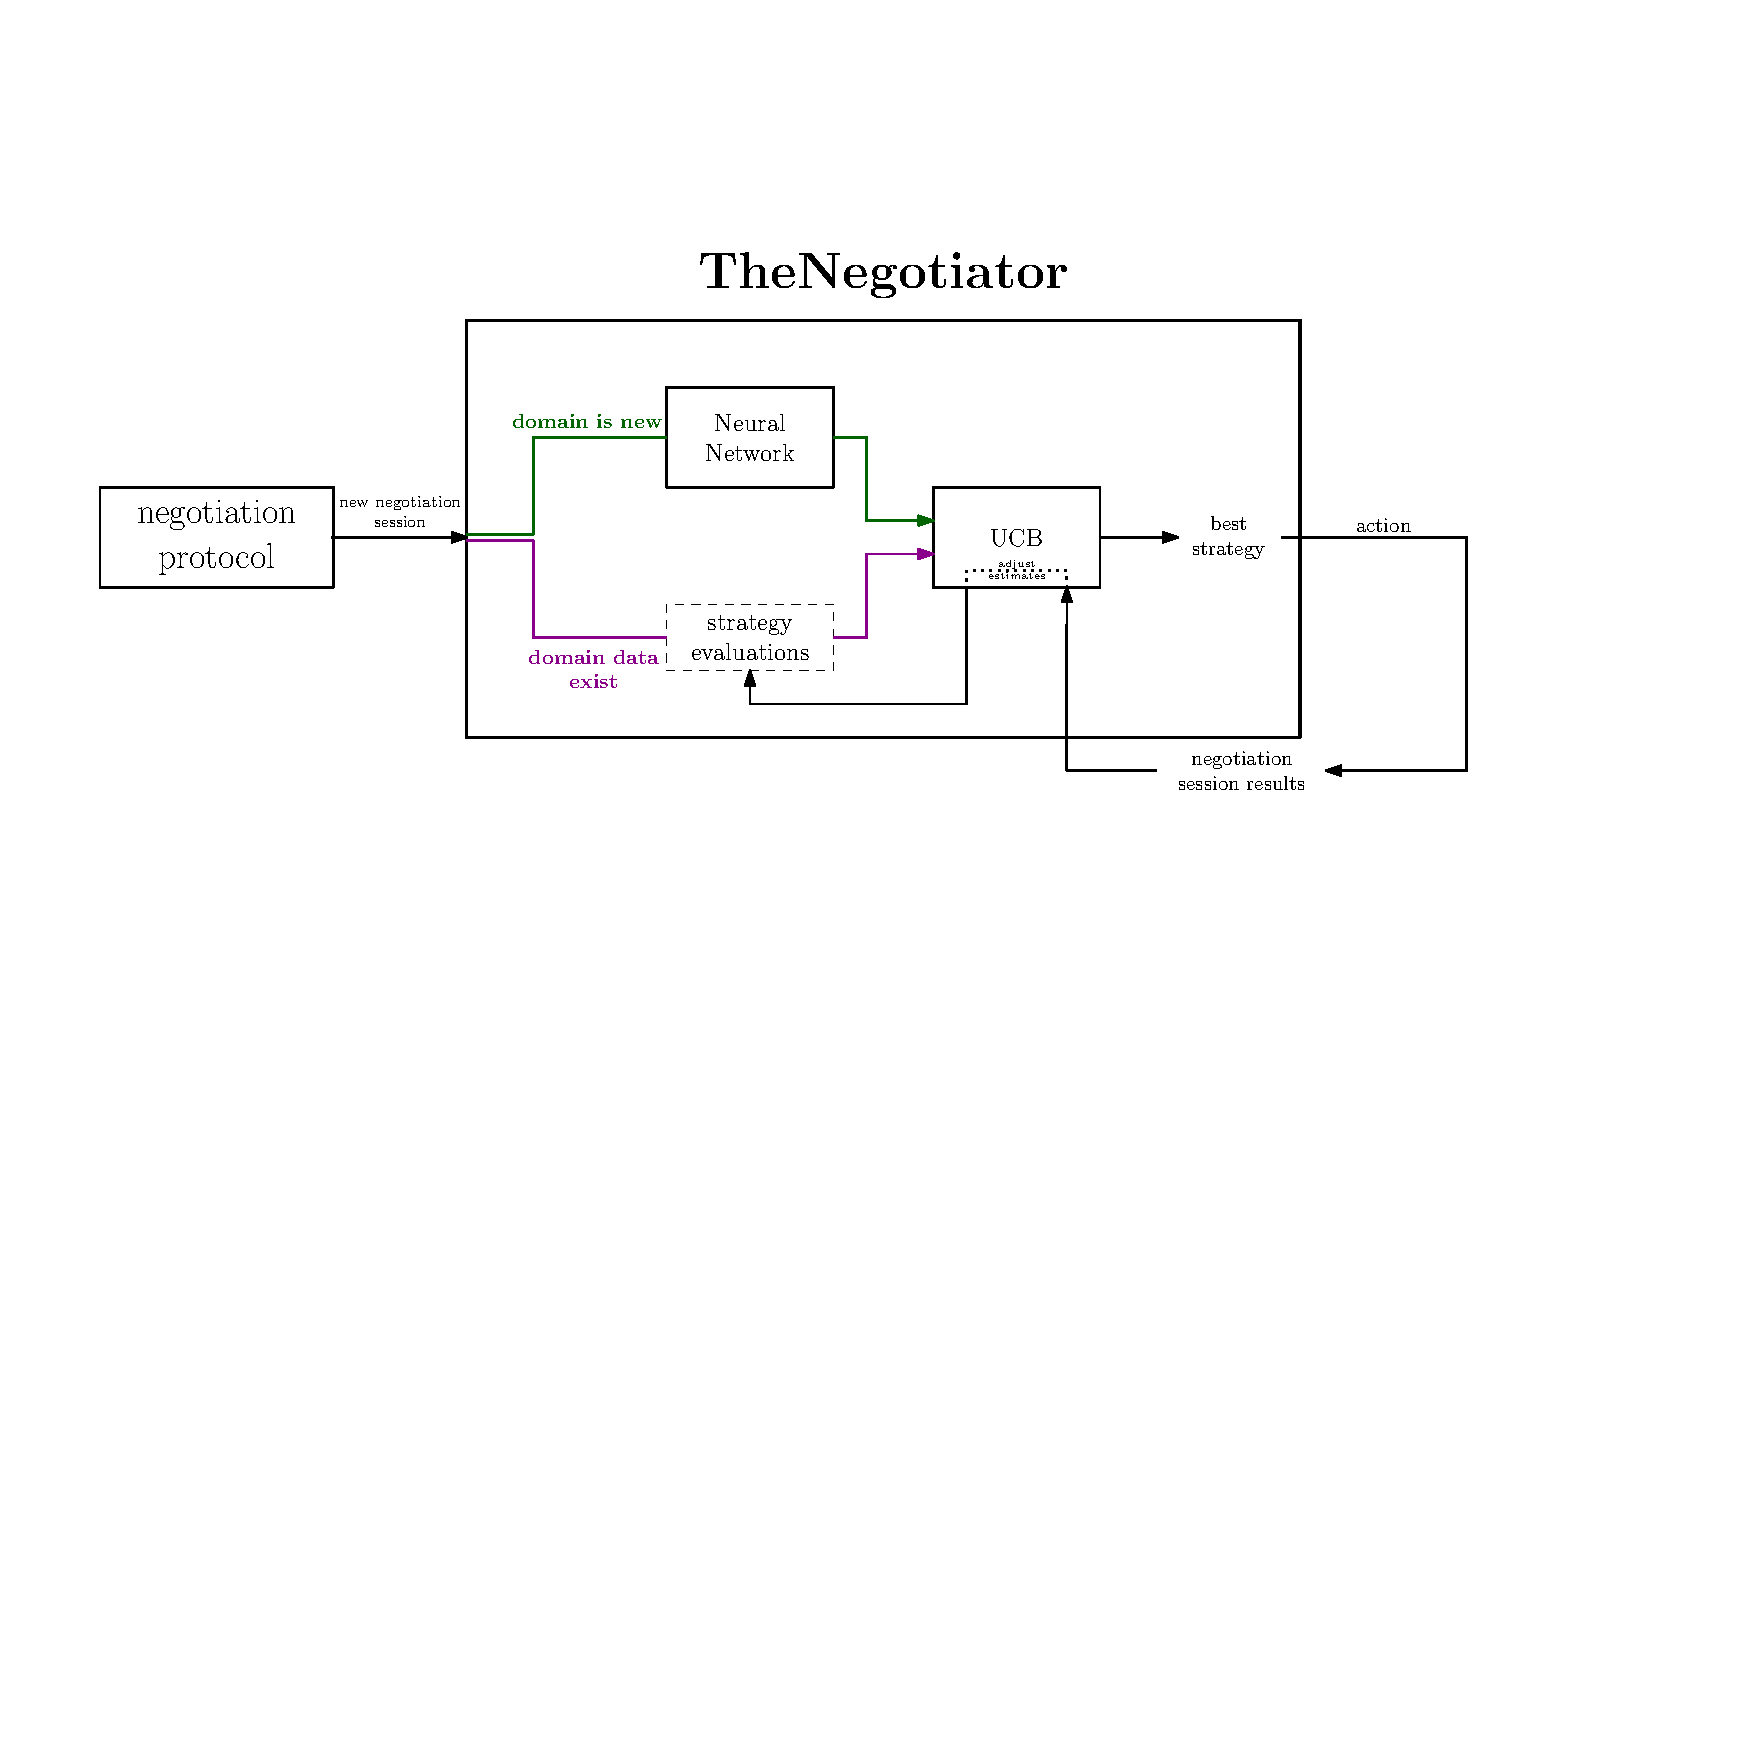
\includegraphics[scale=0.5]{high_level_overview.pdf}}
\captionsetup{justification=centering}
\caption{A high-level overview of TheNegotiator's function}
\label{fig:high_level_overview}
\end{figure}


		\subsection{Using Other Agents}		\label{sec:implementation.using_other_agents}

			
\paragraph*{}
The agents we chose to populate our arsenal were picked from the ANL2022 contestants and CSE2310 agents (available \href[]{https://tracinsy.ewi.tudelft.nl/pubtrac/GeniusWebThirdParties/browser/ANL2022}{here} and \href{https://tracinsy.ewi.tudelft.nl/pubtrac/GeniusWebThirdParties/browser/CSE3210}{here} respectively) based on individual performance and group versatility. Agents' performance was of course a factor, but versatility (in the sense that agents' strategies should vary) was also considered, since similarities in strategy would mean similar strengths and weaknesses, and thus choosing between them wouldn't make much of a difference.
The agents that comprised our arsenal were the following:

\begin{enumerate}
    \item \textbf{GEA\_Agent:} Uses a simple opponent model and a decision tree to find good offers. Uses learning to classify opponents. Implements the BOA framework \cite{BOA_paper}. See \href[pdfnewwindow]{https://tracinsy.ewi.tudelft.nl/pubtrac/GeniusWebThirdParties/browser/ANL2022/gea_agent/ANAC 2022 GEA report.pdf}{here} for more information.

    \item \textbf{DreamTeam109:} The winner of ANL 2022 in both individual utility and social welfare. Also implements the BOA framework. Learns the best time to start compromising versus each opponent. See \href{https://tracinsy.ewi.tudelft.nl/pubtrac/GeniusWebThirdParties/browser/ANL2022/dreamteam109_agent/DreamTeam109 ANL2022 Agent Strategy.pdf}{here} for more information.

    \item \textbf{Agent007:} Uses frequency-based opponent modeling \cite{HardHeaded}. Came in second in the social welfare category of ANL 2022. Observed to achieve very high utilities in experimental tournaments run while exploring the alternatives.

    \item \textbf{TemplateAgent:} Given from ANAC as an example of an agent implementation to help competition participants. Acts like a hardliner for the best part of a negotiation session and starts conceding linearly close to the end. As a result of the hardliner behavior, many opponents may accept its demands before the conceding period begins in order to avoid a disagreement. Observed to perform well in various experiments as well.

    \item \textbf{Agent33:} Alexander The Great. Jesus Christ. Larry Bird.
    % Korydallos Correctional Facilities.
    The number 33 just seems to be inexplicably linked with greatness, and who are we to deny the ways of the universe?	% TODO: ti kanoume edw lol
\end{enumerate}
We refer to agents that TheNegotiator uses as \emph{strategy agents}.

\paragraph*{}
The inquisitive and skeptic reader might have had some thoughts along the lines of \quotes{those agents were made to participate in competitions, not to be used by other agents. Was that not a problem?} \textendash \ and they would be correct. In order to use readily available agents as part of our arsenal we had to make some adjustments to their code. We made the modification process very simple (2 lines of code per agent) since changing arsenal configuration was a crucial part of our process and we had to keep its overhead as small as possible.

\paragraph*{}
The fact that the agents were made to participate in the same competition meant that there was a lot of uniformity in their design, and thus they could all be interacted with in the same way. Since they were all designed to communicate with the same machinery (henceforth referred to as the \emph{protocol}), we had to \emph{be the protocol} as far as they were concerned: we had to do everything the protocol would do if they were in a real tournament. This begs the question of \emph{what does the protocol do}. Basically the process is as follows: it creates the agent (instantiates its class), passing only the path to its storage directory as a constructor argument. The rest of the interactions take place through a method that all agents have to implement, named \texttt{notifyChange} that is called by the protocol whenever something happens, and contains the agent's logic as to how to handle each event. The possible event types are the following:
\renewcommand{\arraystretch}{1.5} % Adjust the value as needed
\begin{longtable}{l p{290pt}}

    \texttt{Settings}: & Happens only once at the start of the negotiation session. Informs the agent of the domain and its profile. \\

    \texttt{Finished}: & Happens only once at the end of the negotiation session. The agent must then free its resources. \\
    
    \texttt{ActionDone}: & Happens each time an agent acts. This is the way agents learn the actions of their opponents. \\
    
    \texttt{YourTurn}:	& Means that the agent must tell the protocol if it accepts the opponent's offer or extend one of its own. \\

\end{longtable}

\paragraph*{}
The way in which one would mimic the protocol is quite straightforward. When we are notified of a new negotiation session (through a \texttt{Settings} event) we will select the appropriate agent and instantiate it, giving it a directory (inside what the protocol gave us) to use for its purposes. Every other event can just be passed to the strategy agent as-is, and it will do its thing. However, in the case of a \texttt{YourTurn} event, the way the agent sends its action to the protocol is not so straightforward, and thus requires a more intrusive approach.

\paragraph*{}
The way the agent sends its action to the protocol is the following (see \cref{fig:protocol-agent_connection}):
\begin{enumerate}
    \item When the agent is created, the protocol \emph{connects} with it: a two way socket-like connection is established, that can be used to exchange data between them. \footnote{Agents are actually just listeners on this connection, and \texttt{notifyChange()} is just the callback function.}
    
    \item When a \texttt{YourTurn} event is received and the agent's logic has produced an action, it is sent to the protocol through that connection.
\end{enumerate}
Luckily, the only time agents may need to send data to the protocol is at the end of a turn. This means that we are free to override this connection from the agent's side and intercept any data going through it.

\begin{figure}[H]
\centering
\framebox{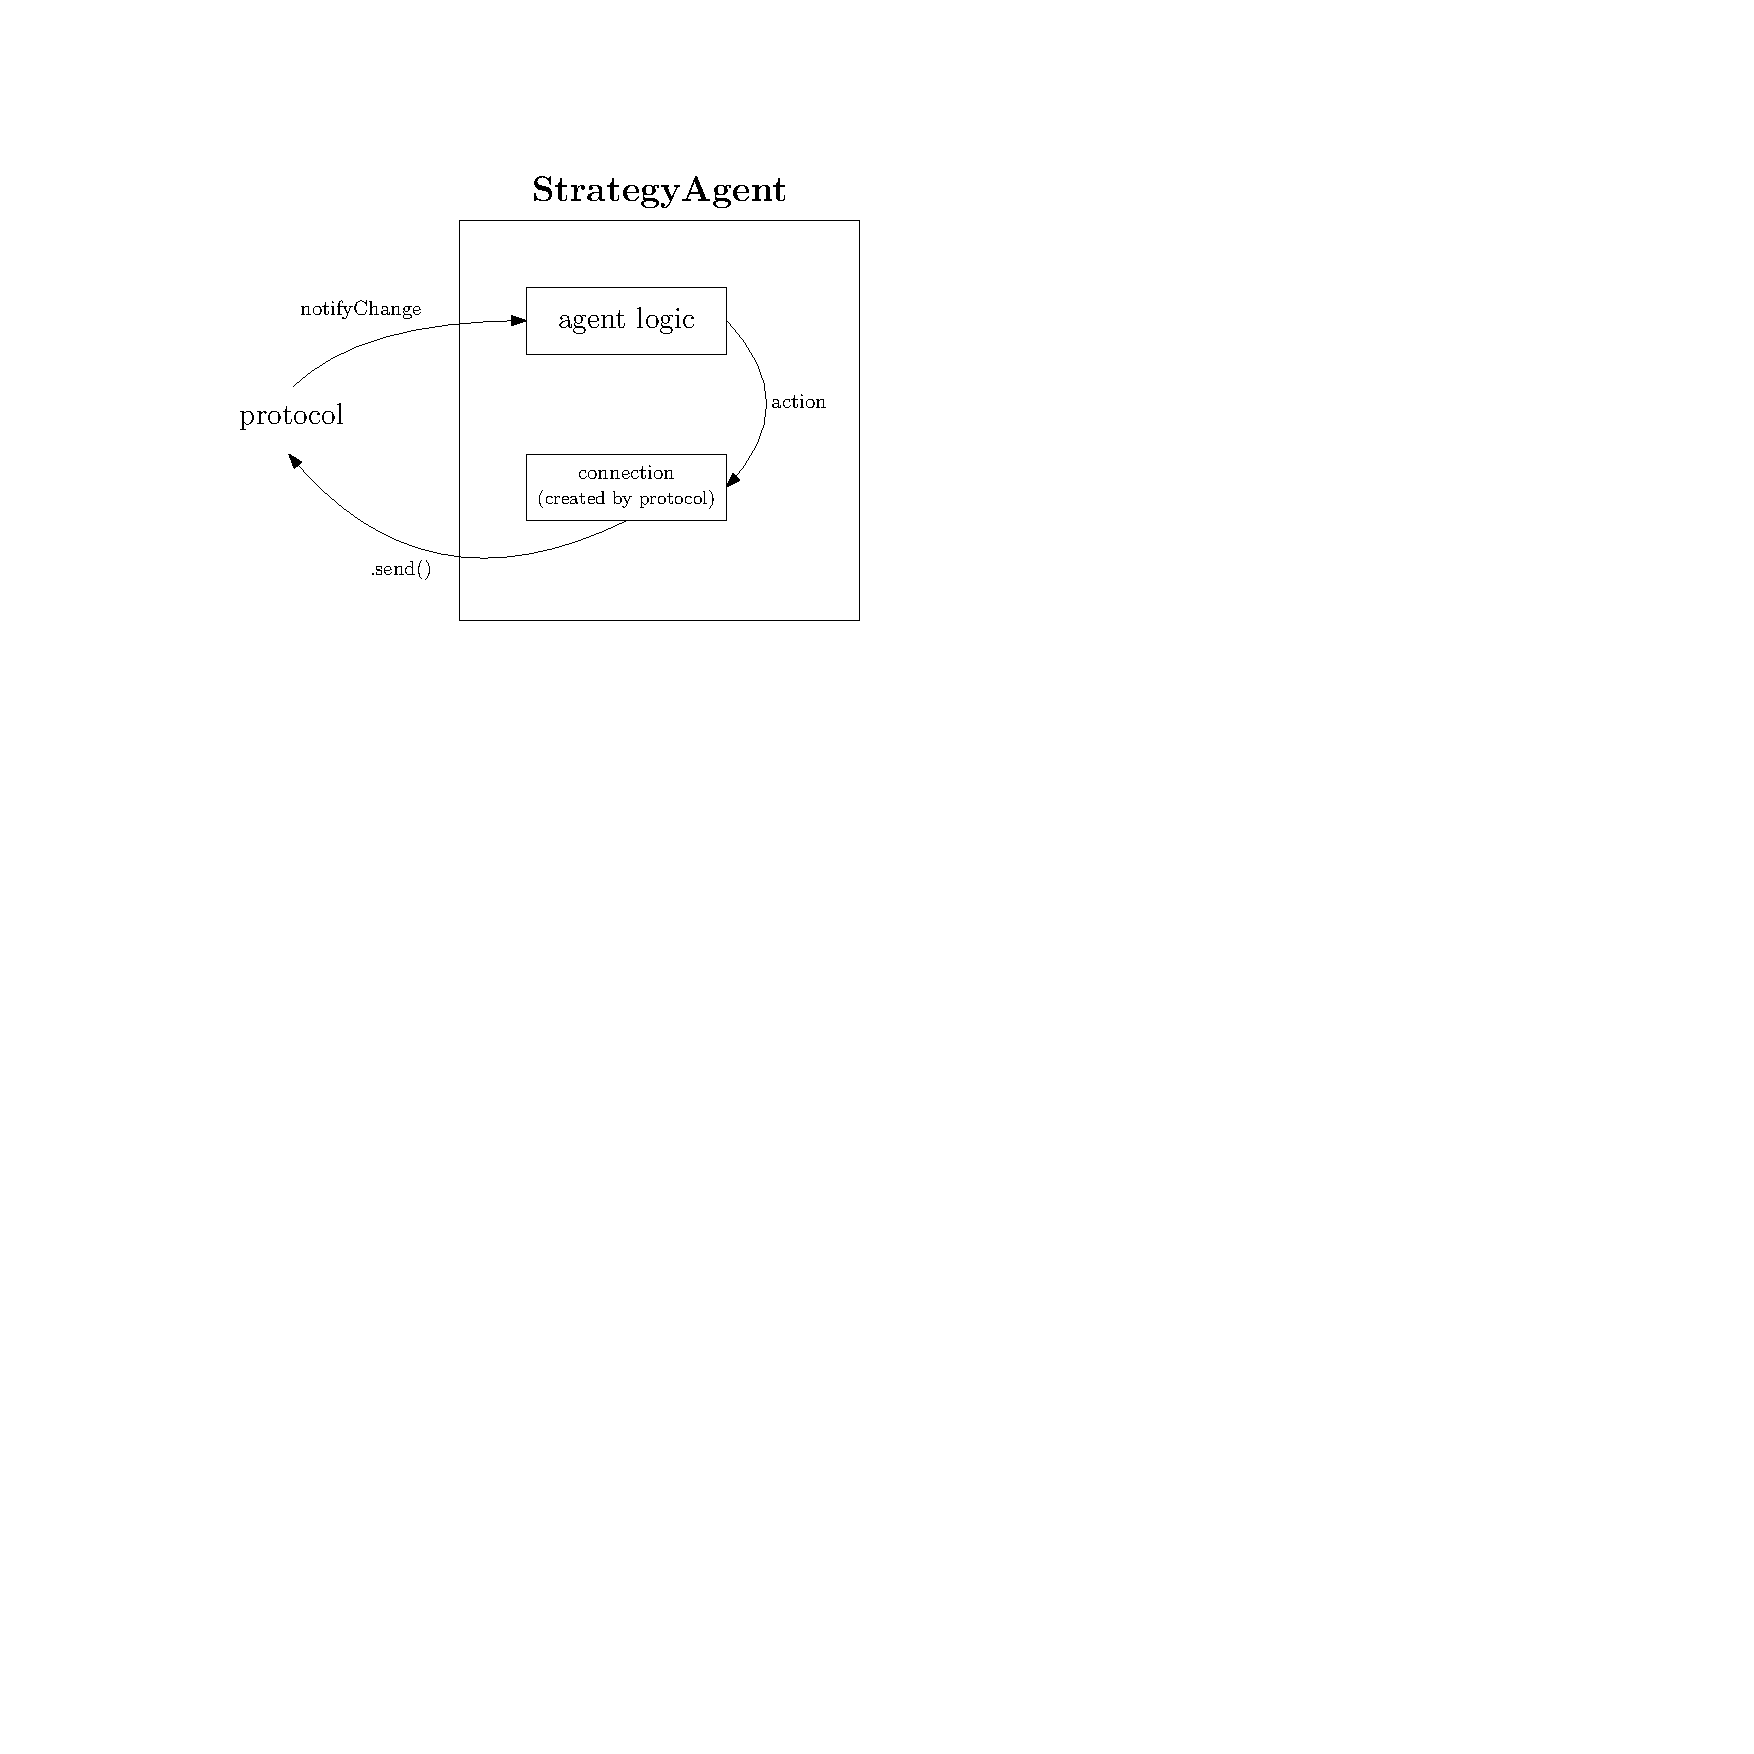
\includegraphics[scale=0.5, page=1]{mixin_explainer.pdf}}
\captionsetup{justification=centering}
\caption{The communication between the protocol and a generic agent}
\label{fig:protocol-agent_connection}
\end{figure}


\paragraph*{}
Unfortunately the way the protocol establishes this connection is quite complicated, so much so that using it to establish a connection between TheNegotiator and the strategy agent is neither guaranteed to work nor worth the hustle. % h zwh me ekane hustla
Our approach (see \cref{fig:agent-agent_connection}) was extremely simple, and based on the fact that the connection is just an attribute of the agent, and as such can be overwritten easily.

\paragraph*{}
We created a \texttt{CustomConnection} class that mimics the connection at the agent's end. Objects of this class are linked with a proxy when created, and when \texttt{send()} is called, they just copy that data to an attribute of the proxy.

\paragraph*{}
In order to \quotes{plant} the custom connection in the agents we want to use, we created the \texttt{ConnectionInterceptMixin}, that offers two methods. One is used to override the connection's \texttt{get()} method and return the custom connection instead of the real one. The other one lets TheNegotiator set itself as the proxy, giving it access to all the data sent through that connection. All one then has to do to make an agent usable by TheNegotiator is make it include the \texttt{ConnectionInterceptMixin}.

\begin{figure}[H]
\centering
\framebox{\includegraphics[scale=0.5, page=3]{mixin_explainer.pdf}}
\captionsetup{justification=centering}
\caption{The communication between the protocol and TheNegotiator using a strategy agent}
\label{fig:agent-agent_connection}
\end{figure}



		\subsection{Offline Learning - Neural Network}		\label{sec:implementation.neural_network}

			\paragraph{}
A different strategy might perform better in one domain and worse in another.
Our goal was to find the correlation of the domain characteristics with the performance of each of the agents in our arsenal in that domain, in order to choose the one that will theoretically give us the best utility. 

\paragraph{}
 First we needed to collect data that will give us insight about the performance of each agent in a given domain. 
 This was handled by a custom runner, that ran negotiation rounds and stored the utility in files.
 \paragraph{}
 We set a negotiation setting with 5 agents in the arsenal, 10 opponents and 45 domains, meaning approximately 4500 negotiation rounds and approximately
10 hours of runtime (split into multiple computers by running the negotiations in separate domains in the same time).
\paragraph{}
 From this data we collected the average utility (the negotiation rounds with 10 opponents ) of each of the 5 agents and the characteristics of the domain. 
 The characteristics of the domain that we used are:
\begin{itemize}
	\item {Average bid utility} 
	\item {Average number of values per issue}
	\item {Bid utility standard deviation}
	\item {Number of bids}
	\item {Number of issues}
	\item {Weight Standard Deviation}
  
\end{itemize}

\paragraph{}
 The next logical step in order to handle this data is to use Machine Learning. Multiple viable methods exist 
 like CART which was the algorithm of choice for the Research Paper, along with others like Regression methods and a Neural Network , 
 but we decided to use a Neural Network (albeit with a different architecture) , because we were confident that this would be an effective, simple and efficient approach. 
 \paragraph{}
 In our problem the Neural Network 
 is a scalable solution because if the dataset becomes bigger, with more negotiation rounds, 
 the training time scales up, but we do not need to “carry” a huge dataset or retrain the model from scratch each time new data comes in, 
  neither is the structure itself growing in disk size. All we need to do is a training step for the new data, which consists of a forward pass with backpropagation.
\begin{figure}[H]
\centering
% First picture
\framebox{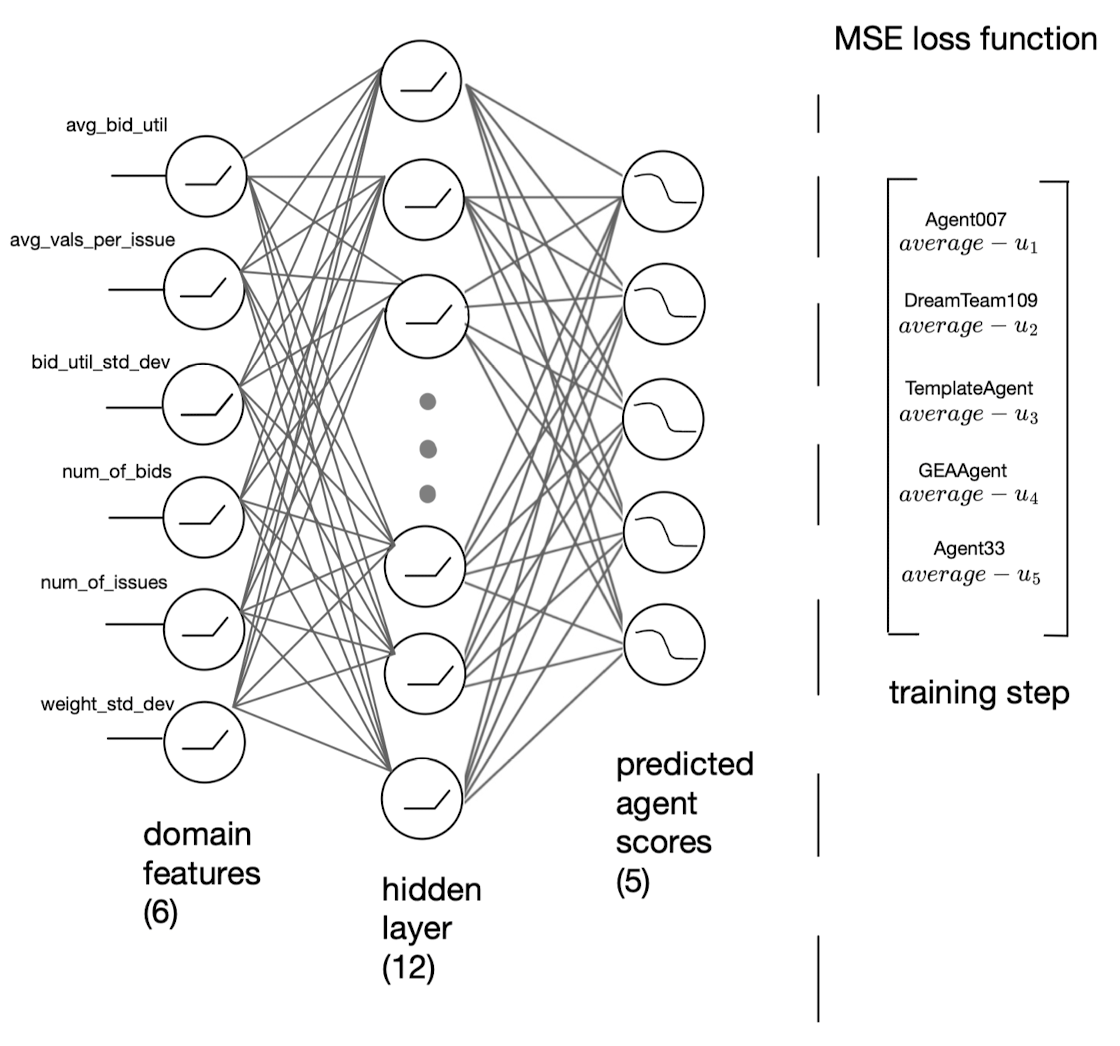
\includegraphics[scale=0.45]{nn_train.png}}
\captionsetup{justification=centering}
\caption{Neural Network Training}
\label{fig:NeuralNetworkTraining}
\end{figure}


\paragraph{}
 The Neural Network takes the domain characteristics (X) as input data along with the real average utility that the agents gained (Y) from the negotiation rounds in the specific domain. It’s goal is to train the Network (adjusting the weights and biases) so that giving the characteristics of a new domain gives us a prediction of each agent’s performance in it which can be very beneficial.  
 The training happens by passing the domain characteristics in a forwards pass, getting the outputs and using the Mean Square Error loss function to calculate the error between the outputs and the real scores and then using the optimizer, adam in our case to adjust the weights and biases with backpropagation.
 \paragraph{}
 

The architecture of the Neural Network is simple but a bit more complicated than the one decribed in the research paper \cite{meta_agent_paper}, even though not a lot of data is disclosed about it.
 We use an input layer of size 6, for each one of the domains characteristics, 
 a hidden layer of size 12 which is 2 times the size of input layer, in order to be able to detect hidden patterns in the data but showed 
 the best results between the values we tested and an output layer of size 5, for each of the agent's performance.  
 The input and hidden layers used the relu activation function and the output layer used the softmax activation function, which ensures that the outputs are a value between 0 and 1 and is a good fit for our predictions problem. We used 2 epochs for the training because it showed good results with no overfitting, like 3 or more epochs (showing similar results for different input features) and
  more effective training rounds than 1 epoch. Finally a dropout layer was applied (not shown in the figure, between the hidden layer and the output) with a dropout chance of 30\% that works by 
  randomly setting a fraction of input units to 0 at each update during training, which helps to make the model more robust and generalize better to unseen data. 
\paragraph{}



After the training is done to get the predictions for each agents, 
all we need is a forward pass of the domain characteristics from the Neural Network. 
This concludes the off-line training part of the problem, but the scope of the Negotiator does not stop there.
In the next part we test how the output of the Neural Network can give some knowledge to an on-line algorithm 
which will continue the learning with a different approach.
\begin{figure}[H]
	\centering
	\framebox{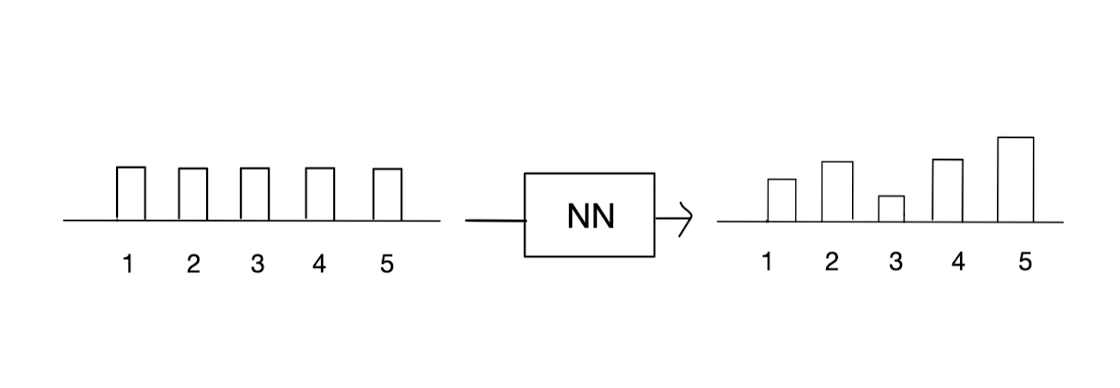
\includegraphics[scale=0.55]{nn_ucb.png}}
	\captionsetup{justification=centering}
	\caption{Setting the initial confidence bounds}
	\label{fig:Setting the initial confidence bounds}
\end{figure}
 
		
		\subsection{Online Learning - UCB}		\label{sec:implementation.ucb}

			\paragraph*{}
In the previous section we described how the neural network that provides us with the initial performance estimates works. However, if that was all our agent did, an error in its output would mean that we're stuck with a sub-optimal agent for all sessions in a certain domain. % TODO: better way to say it
Luckily, we can observe the result of each session \textendash \ the utility we gained  \textendash \ and we can judge if our estimates are correct or if they need adjusting.

\paragraph*{}
To do that, just like \cite{meta_agent_paper}, we model the competition as a Multi-Armed Bandit (MAB) setting, as defined in \cite{MAB_Lai_Robbins_1985} and \cite{MAB_paper_2002}: we have several agents in our arsenal (the \emph{arms}) and in each negotiation session (a MAB \emph{round}) we pick one and gain some utility (\emph{reward}). Such settings are well studied in the Reinforcement Learning (RL) literature and many algorithmic approaches exist to solving them. % TODO: language

\paragraph*{}
Of those algorithms we chose the Upper Confidence Bound (UCB) \cite{UCB_paper} mainly for the following two reasons: Firstly, it offers a theoretical upper bound  on \emph{regret}\footnote{regret is the difference in utility between the optimal choice in each round and the one we played, i.e. $u_{opt} - u_{picked}$. The optimal choice is not actually calculated since we do not wish to measure regret, but it can be computed by playing all alternatives and picking the best.}, which is guaranteed to be sublinear (specifically $O(\sqrt{T})$, where $T$ is the number of rounds played). Secondly, it is very simple to implement and experiment with. % TODO: maybe a closing sentence?

\paragraph*{}
The way UCB works is the following:
\begin{itemize}
    \item We maintain an array \texttt{ucb} with one element for each agent in the arsenal representing our \emph{opinion} of that agent, i.e. the utility we predict it will achieve.

    \item Our opinion of an agent \texttt{a} in our arsenal is defined as the sum of a \emph{performance term} \texttt{p} and a confidence bound \texttt{c}, i.e. $\texttt{ucb[a]} = \texttt{p[a]} + \texttt{c[a]}$.

    \item The performance term \texttt{p} is initially set to the NN's output, and is then adjusted each time \texttt{a} is picked to include the new information we gained about it (how well it did).
    
    \item The confidence bound \texttt{c} reflects \emph{how confident we are in the correctness of the performance term}. If we are very confident, then this term is low, since \emph{we cant be far off}. Confidence is only related to the number of rounds in which \texttt{a} was picked and the number of total rounds played. The more times we have picked \texttt{a}, the more confident we are that \texttt{p[a]} is accurate.

    \item In each round, we pick the agent with the highest \texttt{ucb} score.
\end{itemize}
Notice that if we are not very confident about an agent \texttt{a}'s performance \texttt{c[a]} is high, meaning \texttt{ucb[a]} is also high, and thus \texttt{a} is likely to be picked. For this reason UCB is characterized as \quotes{optimistic}, in the sense that we evaluate the alternatives based on how well they \emph{might} do, pick the one that might do the best and \emph{hope} that it does.

\paragraph*{}
To better explain this idea we provide an example. Suppose that TheNegotiator is about to negotiate in a previously encountered domain. Suppose also that the \texttt{ucb} array for that domain is depicted in \cref{fig:UCB_example}. TheNegotiator would then pick agent 1, as it has the greatest sum of performance and confidence terms, even though the performance term $p$ of agent 4 is higher. This demonstrates the optimism of UCB: it makes its decision \emph{as if} agent 1 will be the best it can be and outperform agent 4.

\begin{figure}[H]
    \centering
    \framebox{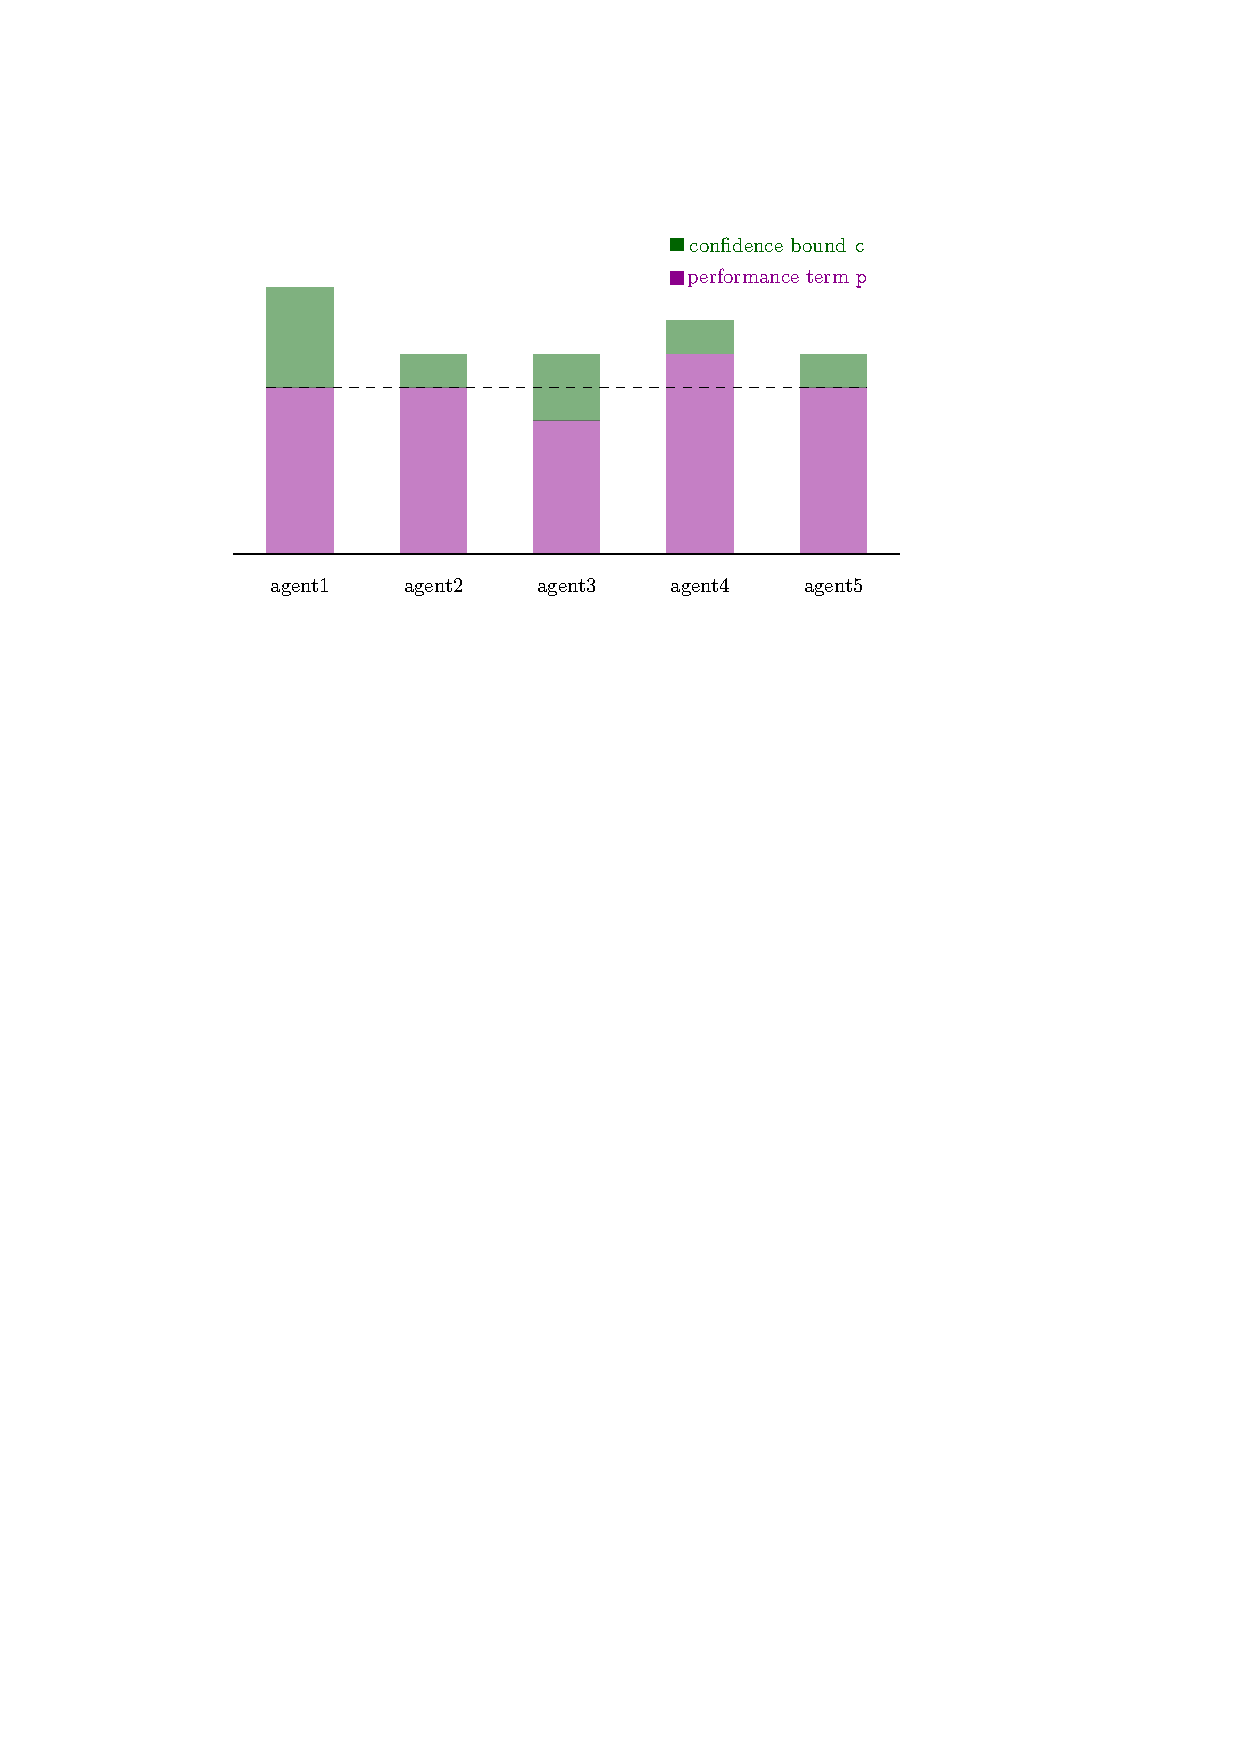
\includegraphics[scale=1, page=1]{ucb_demo.pdf}}
    \captionsetup{justification=centering}
    \caption{An example of UCB for 5 agents}
    \label{fig:UCB_example}
\end{figure}

\paragraph*{}
The process described above is done for every domain, since each domain is treated as its own, separate environment. Since a different instance of TheNegotiator takes part in each negotiation session, the UCB arrays have to be stored on disk. A subdirectory inside the given agent storage was used for that purpose, with a file for each combination of domain and preference profile (e.g. \texttt{domain07\_A.ucb} and  \texttt{domain07\_B.ucb} would both correspond to domain 7, but the first one would be for when we are given profile A and the second for when we are given B).

\paragraph*{}
Mathematically, the logic above is expressed like this:
\begin{equation} \label{eq:UCB}
    {ucb_{a}}' \quad = \quad \underbrace{\frac{[ucb_{a} \cdot (n_{a}-1)]+u}{n_{a}}}_{\texttt{p[a]}} \quad + \quad \underbrace{\sqrt{\frac{2 \ln N}{n_{a}}}}_{\texttt{c[a]}},
\end{equation}
\vspace{-0.5cm}		% brings the table a bit closer to the equation
\renewcommand{\arraystretch}{1} % Adjust the value as needed
\begin{longtable}{l l l}
    where 	& ${ucb_{a}}'$	& is the updated value of \texttt{ucb[a]} after picking it in the last round, \\
            & $ucb_{a}$  	& is the previous value of \texttt{ucb[a]}, \\
            & $n_{a}$ 		& is the number of times \texttt{a} has been picked, \\
            & $u$ 			& is the utility achieved in the last round by \texttt{a}, and \\
            & $N$ 		& is the number of total rounds played. \\
\end{longtable}

\paragraph*{}
The reader might also notice a problem with the UCB formula in equation \ref{eq:UCB}: on initialization, since $n_{a}=0$ for every agent $a$, all values in the UCB array will blow up to infinity. This is in fact intentional, as it forces the agent to play as every agent at least once, thus obtaining a an actual result from it in order to enhance/correct the neural network's prediction.


	\section{Results}		\label{sec:results}	% edw tha mporousan na paiksoun kai ta logs kalo rolo
	\paragraph{}
 The Negotiator agent was able to participate in the Technical University Of Crete competition and win the 2nd place. This proves that the meta agent strategy is effective in negotiations with diverse agents.
The UCB algorithm is effective in making the Negotiator adaptive, but also the prior knowledge from the Neural Network gives it a substancial headstart. As the research paper 
\cite{meta_agent_paper} stated, a little learning does indeed go a long way.
\paragraph{}
The results that the Neural Network produced seem logical and it manages to capture the corellation between the characteristics of a domain and the optimal agent, with our preliminary testing. As seen in the log files
of the competition and as tested the UCB algorithm works correctly, adjusting as expected after each round.

 
	\section{Limitations \& Improvement Proposals}		\label{sec:limitations_improvements}
	
		\begin{itemize}
			\item We would ideally want more testing to happen to see how this strategy (meta agent) with this specific set of strategy agents performs on different domains.
			\item We are interested in testing different on-line algorithms and variations instead of UCB to differentiate our work from the research paper \cite{meta_agent_paper} and maybe get better performance.
			\item In the TUC competition we had a very limited number of opponnents which limits tha UCB algorithm, giving it less rounds to work.
			\item We did not implement an opponnent modeling system, instead basing our learning only on domain characteristics.
			\item Implementing such a system or using machine learning on different opponent behaviors would be a logical next step.
			\item For the competition we used 5 different strategy agents because we wanted The Negotiator to be able to have different behaviors on demand. Further research on the different types of used agent behaviors and checking whether more or less agents have better results would be beneficial. 
			\item In the transition from the off-line to on-line learning we set the Neural Network training to count as 10 rounds of UCB (for arithmetic and logical reasons).
			\item We tried changing the above to other values like 20 rounds but did not get better results.
		\end{itemize}

	\bibliographystyle{plain}
	\bibliography{refs}


\end{document}